%!TEX root = ../report.tex

% 
% Introduction
% 

\section{Introduction}

%General description of the problem and its context, current solutions, and road map of the project.

%This days designers and developers have available a large number of Computer Aided Design(CAD) tools to produce their models. This tools are getting more and more powerful and with more features available. The traditional way of modeling where the user adds geometry one by one does not present performance issues about rendering. On the other hand it is being more and more common the concept of generative design, that is a design method that is based on a programming approach which allows architects and designers to model large amounts of shapes with significantly less effort.

As technology evolves people have more powerful devices and they want to take advantage of that. They want to have more realistic experiences with larger, more detailed and complex contents.
And this is observable in the graphic contents. With the recent extra high definition on screens and the computational power of the machines beating records, the graphic content has to follow up that characteristics in quantity as well as in quality. The issue is that the manual content generation takes a long work time from architects and designers to achieve this quality, thus implying high costs.

Graphic contents are mainly used for entertainment, both in the gaming and movie industries, but it is also used in a lot more different areas. The fields of architecture and design, for instance, use this technology to experiment and model new designs, from small objects like a plate to buildings or even entire cities. In this field they also face the problems that raises from the modeling of really big sets of objects and forms manually. \emph{This work focus on this problem of content creation for the fields of architecture and design.}

The obvious answer to this problem of manual content creation costs is to contract more architects or designers to each project to increase the production, but experience have shown that this solution is not scalable, that means that double the number of architects or designers working in a project will not double their overall productivity. Also this solution has a big impact on costs, that would take immediately out of the market new producers with less resources.

A solution for this problem is the use of generative design. That is a design method that is based on a programming approach which allows architects and designers to model complex shapes with significantly less effort. 

Although most computer-aided design (CAD) applications provide programming languages for generative design, programs written in these languages have very limited portability. This languages, such as AutoLisp, C++ or Visual Basic, are not pedagogical and are difficult to use even to experienced programmers, problems that create barriers to adherence to this approach by users specially to those that normally are not used to code.\cite{ramos_et_al:OASIcs:2014:4565}

There are several generative design (GD) tools such as Grasshopper\footnote{\url{http://www.grasshopper3d.com/}} and Rosetta that aim to break down some of this barriers and facilitate the approximation of these individuals to programming. With this tools the users create their models with pedagogical and easy to use languages. This systems implement a straightforward pipeline presented in Figure~\ref{fig:GD_Pipeline}. 

One big difference from traditional approaches is that the users do not see the result of their program while they code. They should follow a code-execute-visualize loop where they make changes in the code, execute the code and visualize the resulting model. They also want to easily understand the correlation between their program and the resulting model and to be able to experiment values on their program and see the effects they have on the model. To help them with this there is the concept of \emph{immediate feedback}. Immediate feedback is a mechanism that allows the users to see the results of the changes they make in the resulting model. This can be implemented, for instance, through the use of sliders that can be associated with values on the program, and when one slider is moved the effects of that change should be visualized immediately. 

\begin{figure}[htbp]
	\centering
	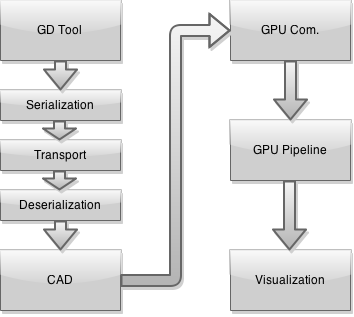
\includegraphics[width=0.45\textwidth]{img/Architecture/GD-Common-Pipeline.png}
	\caption{Common Generative Design Pipeline}
	\label{fig:GD_Pipeline}
\end{figure}

%\begin{wrapfigure}{r}{0.5\textwidth}
%	\vspace{-15pt}
%    \centering
%	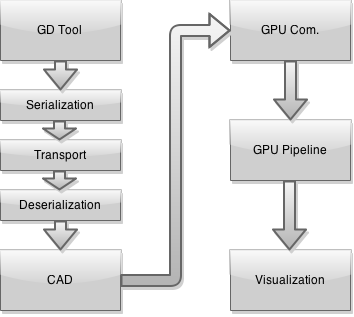
\includegraphics[width=0.5\textwidth]{img/Architecture/GD-Common-Pipeline.png}
%	\caption{Common Generative Design Pipeline}
%	\label{fig:GD_Pipeline}
%	\vspace{-15pt}
%\end{wrapfigure}

With this rises the problem of performance. The architects and designers implement their models on GD tools that generate the geometry. Then, as Figure~\ref{fig:GD_Pipeline} shows, the all geometry data is serialized and the data is transfered through sockets. This data have to be deserialized on the other side within the CAD application. This CAD application takes the objects and processes them adding their specific information to the geometry. At last the geometry is moved to the GPU that renders the model. All this steps are time-consuming mostly caused by the large amount of data that is repeatedly transfered. There is also another problem, CAD applications are built for manual modeling mainly, and are not prepared to receive large amounts of geometry very fast. Running the code is much faster than manual modeling, so the user is able to create massive amounts of geometry fast that is fed to the CAD that gets overloaded. With this issues, it is hard to get good performance, specially with large models, that makes impossible to have true immediate feedback. Users sometimes have to wait a lot of time for the model to be rendered.

%There is a tool that aims to break down some of this barriers and facilitating the approximation of these individuals to programming. It is \textbf{Rosetta}, an extensible IDE based on \textbf{DrRacket} and target at architects and designers.\cite{lopes2011portable} The users specify their models in Rosetta that generates the geometry and transports all this data to the CAD tool that then moves the data to the GPU to graphics visualization. Rosetta works with various CAD tools because it also have interoperability as a special concern. 

% if with each small change they have to wait a significant amount of time it have a significant impact for the work of the designers. 

%There is an area of research that addresses this problem named \emph{Procedural Content Generation}, or \emph{Procedural Generation}. This have applications for example in the creation of large and/or complex scenarios for games and movies or the creation of models to use for simulation of cities. This examples involves the generation of large amounts of forms that would be impracticable with the manual approach to content creation.

This work proposes a solution to this problem. It does so by jumping over some steps while drastically decrease the amount of data that is transfered between steps. First we aim to get the geometry as fast as possible to the GPU, so since our goal is just visualization we jump the CAD layer and with that eliminate the communication connected with it. Another action is to reduce the amount of data that is transferred and it is achieved by transferring only a very concise description of the geometry that is generated only on the GPU. To implement the generation of the geometry, procedural techniques will be studied and applied.

